% !Mode:: "TeX:UTF-8"

\chapter{语义分割的应用}

图像语义分割(semantic
segmentation),从字面意思上理解就是让计算机根据图像的语义来进行分割。语义分割是在像素级别上的分类,属于同一类的像素都要被归为一类,因此语义分割是从像素级别来理解图像的。语义在语音识别中指的是语音的意思,在图像领域,语义指的是图像的内容,对图片意思的理解;分割的意思是从像素的角度分割出图片中的不同对象,对原图中的每个像素都进行标注。

\section{地理信息系统}

可以通过训练神经网络让机器输入卫星遥感影像,自动识别道路,河流,庄稼,建筑物等,并且对图像中每个像素进行标注。(左边为卫星遥感影像,中间为真实的标签,右边为神经网络预测的标签结果)
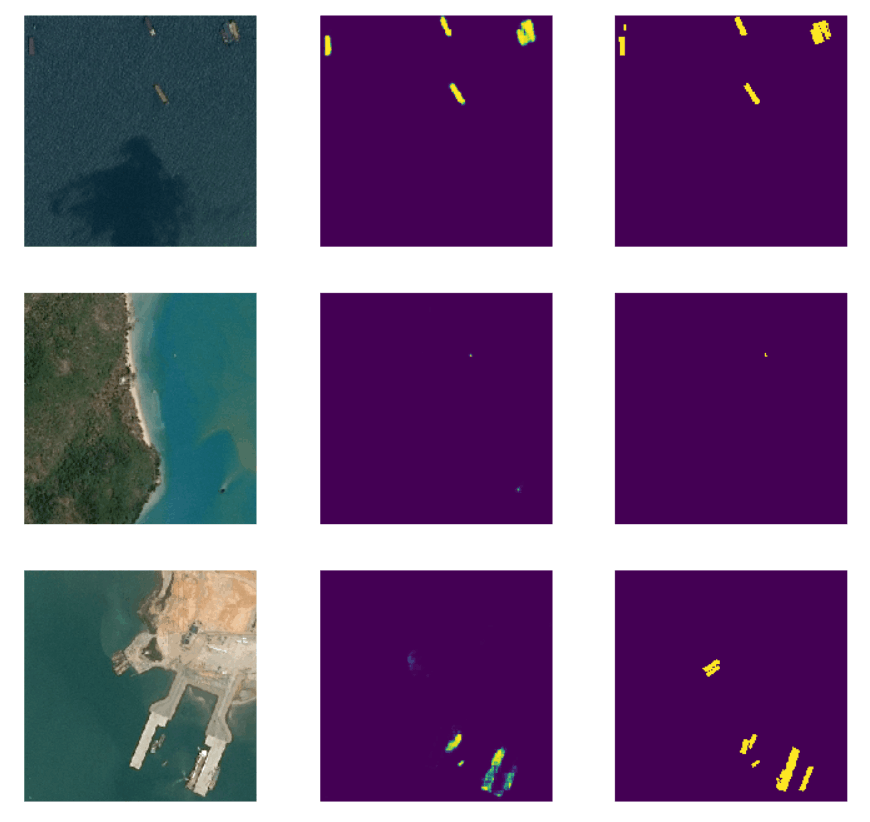
\includegraphics{picture/1.png}神经网络预测的卫星遥感影像

\section{面部分割}

面部的语义分割通常涉及诸如皮肤、头发、眼睛、鼻子、嘴巴和背景等的分类。面部分割在计算机视觉的许多面部应用中是有用的,例如性别、表情、年龄和种族的估计。
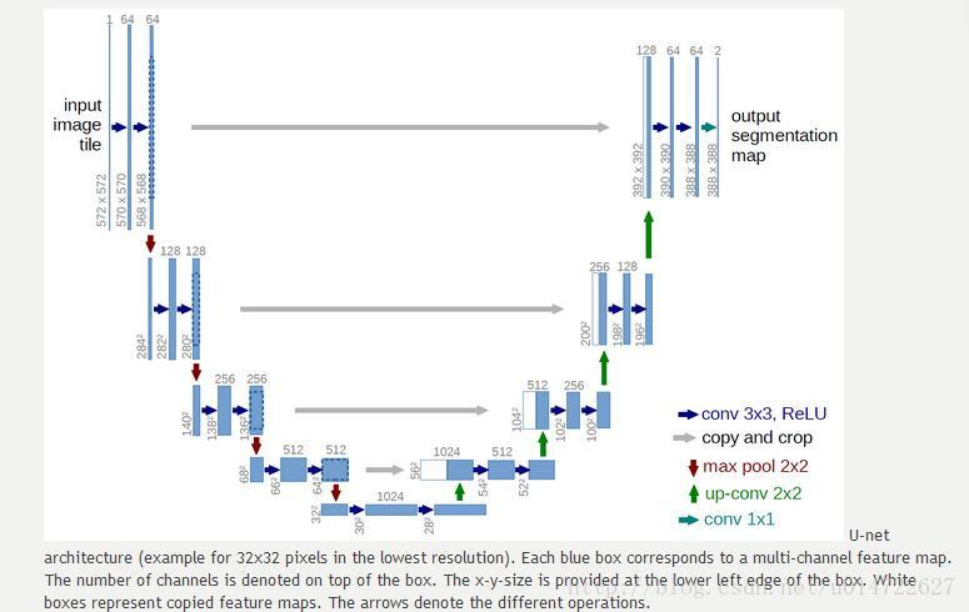
\includegraphics{picture/2.png}神经网络预测的面部图像

\section{无人车驾驶}

语义分割也是无人车驾驶的核心算法技术,车载摄像头,或者激光雷达探查到图像后输入到神经网络中,后台计算机可以自动将图像分割归类,以避让行人和车辆等障碍。
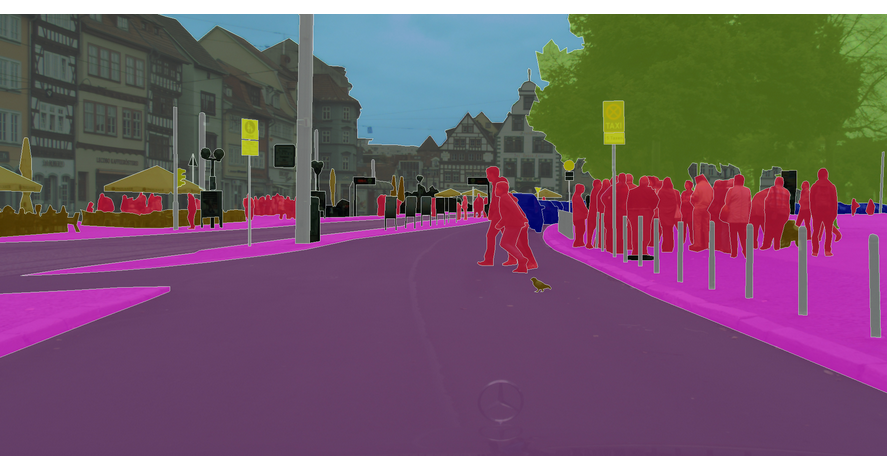
\includegraphics{picture/3.png}神经网络预测的雷达影像

\section{医疗影像分析}

神经网络与医疗诊断结合也成为近期研究热点,智能医疗研究逐渐成熟。在智能医疗领域,语义分割主要应用有肿瘤图像分割,龋齿诊断等。
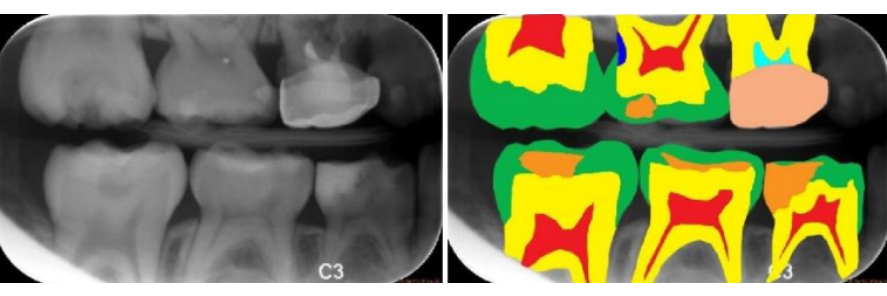
\includegraphics{picture/4.png}神经网络预测的龋齿影像
